\section{Simuladores de realidad virtual}
\label{art:simulador}
\todo{He metido cambios en la intro y en la sección 1.1 sin el control de cambios. Creo que es peligroso (aunque son muy pequeños). A partir de ahora resaltaré toda la frase aunque el cambio sea mínimo.}

\begin{figure}[h]
   \centering
    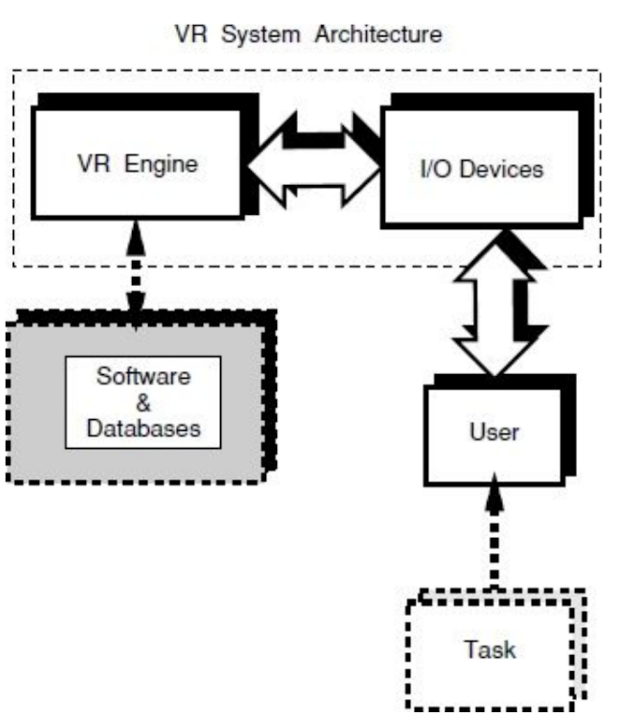
\includegraphics[width=0.5\textwidth]{IMG/VRarq.PNG}
    \caption{Arquitectura propuesta en \cite{burdea2003virtual}. }
   \label{fig:RVarq}
\end{figure}

Según \emph{Burdea y Coiffet}\cite{burdea2003virtual}, un sistema de \ac{RV} se puede dividir en cinco componentes tal y como se puede observar en la figura \ref{fig:RVarq}. En ella, se puede observar las distintas interacciones que se producen entre estos componentes. De manera separada, estos componentes pueden existir independientemente pero, es la relación que existe entre ellos, la que conforma un sistema de \ac{RV}. A continuación, se describirá cada uno de ellos:
\begin{itemize}
    \item Motor de \ac{RV}: Este componente se encarga de realizar los cálculos necesarios para simular la escena virtual. Para actualizar el estado de la escena virtual es necesario que se consulte las bases de datos  y actuar según la entrada recibida a través de los dispositivos realizada por los usuarios. El motor generará y mostrará el nuevo estado de la escena a través de los dispositivos de salida (que pueden incluir más de un canal sensorial). Además, es preciso asegurar una tasa de refresco interactiva. El término motor de RV no se puede asociar a un computador, sino que se tiene que tratar como una abstracción ya que puede tener múltiples configuraciones hardware como puede ser un único computador o un sistema distribuido conectado por red.
    \item Dispositivos de \ac{E/S}: Este componente lo forman todos los dispositivos que utilice el usuario en su interacción con el sistema. Es imprescindible para un sistema de \ac{RV}  que se permita la interacción del usuario. Los dispositivos de entrada se encargan de recoger las acciones que realiza el usuario, mientras que los dispositivos de salida muestran la respuesta de la escena virtual a través de los distintos canales sensoriales. Actualmente, estos dispositivos son muy numerosos y diversos.
    \item Componentes software y base de datos: Este módulo contiene todas las especificaciones y descripciones que caracterizan el sistema. Aquí se incluyen la escena virtual y su organización. \new{Análogamente a una base de datos tradicional, donde se consulta y se recoge información, el esto módulo recoge toda la información necesaria para la simulación.} Además, aquí se incluyen, por ejemplo, las aplicaciones que se diseñan con el objetivo de guiar y facilitar el entrenamiento al dirigir la simulación según la interacción del sistema y el usuario.\todo{Rehaz la última frase.}
    \item Usuario: \new{El principal objetivo de la \ac{RV} es presentar al usuario una escena virtual que este perciva como una representación plausible de la realidad. En este sentido, el usuario y la forma en que este percibe e interactúa con el mundo son componentes clave que hay que tener en cuenta a la hora de diseñar cualquier aplicación \ac{RV}} \del{Es natural que los sistemas se diseñen con el objetivo de que una persona interaccione con ellos. Esta comunicación se realizará a través de los dispositivos de \ac{E/S}}. 
    \item Tareas: Por último, son las tareas, objetivos e instrucciones que se le dan al usuario cuando va a utilizar el sistema de \ac{RV} que le dan significado y utilidad \new{a la aplicación}. Es lo que le diferencia de ser un computador con periféricos conectados de una plataforma de \ac{RV}.
\end{itemize}

\new{En este documento se utilizará esta definición de arquitectura en el capítulo \ref{cap:rasim} como apoyo para explicar el simulador \ac{RASim} y sus diferentes componentes}.A su vez, también puede ayudar al lector a hacerse una idea de cómo se han construidos los simuladores que se presentarán en las siguientes secciones.

\subsection{Simuladores para formación médica}
\label{art:medicalsim}

En los últimos años, los simuladores médicos de realidad virtual están tomando una gran importancia en el currículum de los estudiantes, \new{tanto en le campo de la cirugía como en el de otras especialidades}\cite{PATEL2017266.e7}. Se puede observar un incremento de su presencia para el entrenamiento de jóvenes especialistas tanto en hospitales como universidades. Estas herramientas proporcionan al usuario un método seguro y efectivo de entrenamiento\del{, siendo capaces de usarlo tantas veces como sea posible}. 

Aunque los simuladores están cobrando cada vez más importancia, la enseñanza de medicina \new{actual se apoya una gran variedad de métodos de entrenamiento,} que permite al médico adquirir las destrezas necesarias, antes de poder enfrentarse a escenarios reales de manera autónoma. Una forma segura de entrenamiento es la utilización de \emph{fantomas}\footnote{castellanización del término inglés Phantom} \cite{phantomra}. En la figura \ref{fig:phantom} se puede ver el \emph{Blue Phantom™}\cite{BluePH}\new{, diseñado} para la práctica de ultrasonografía. Estos \emph{fantomas} son modelos anatómicos hechos con materiales sintéticos \new{que intentan} replicar el cuerpo humano \new{y sus propiedades de la forma más fiel posible.} En ocasiones, tienen incorporados una serie de sensores que permiten recogida de métricas. A pesar de que son muy populares, tienen una serie de inconvenientes: no son baratos \new{ y se crean} específicamente para una zona anatómica concreta.\new{No es posible usarlos con otro fin que entrenar el procedimiento concreto para le que fueron diseñados}. Además, si en determinadas ocasiones, el usuario tiene que manipularlos como puede ser hacer una incisión o realizar una inyección en el \emph{fantoma}, el modelo sufrirá desgaste con el tiempo.\new{Por último, destacar que estos modelos representan una única variedad anatómica, enfrentandose el medico al mismo escenario una y otra vez.}
\begin{figure}[h]
   \centering
    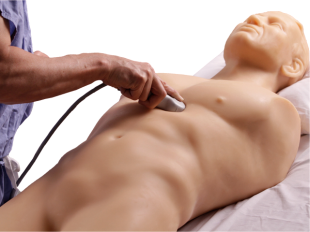
\includegraphics[width=0.5\textwidth]{IMG/fast_trauma.jpg}
    \caption{Maniquí realista para el entrenamiento de ultrasonografía  \emph{Blue Phantom™}\cite{BluePH}. }
   \label{fig:phantom}
\end{figure}

Otra forma de entrenamiento es la utilización de cadáveres\cite{Tsui2007}.\new{Estos permite que el médico se enfrente a casos reales}. En este caso, conseguir diferentes variaciones anatómicas es completamente viable y el mismo cadáver puede servir para entrenamientos de diferentes procedimientos. Aun así, los inconvenientes que presentan son bastante evidentes. Mantener un cadáver en buenas condiciones o que los motivos del fallecimiento hayan perjudicado al estado del mismo, además de ciertos problemas éticos como puede ser el uso de cadáveres procedentes de condenados a pena de muerte (Visible Human Project \cite{ackerman1998visible}).
\todo{Rehaz la última frase. Tambien indicar que la disponibilidad de cadaveres es baja y que no se puede repetir el entrenamiento sobre el mismo paciente. }
Finalmente, los tejidos de un cadáver no muestran el mismo comportamiento mecánico que un tejido vivo, y puede inducir sesgos en el entrenamiento del médico debido a que los músculos se vuelven más rígidos después del fallecimiento \new{el conocido \emph{rigor mortis})}.


La última forma de entrenamiento es la práctica supervisada sobre pacientes reales (\emph{by doing}), donde el estudiante realiza el procedimiento vigilado y guiado por su tutor. Aunque es el entrenamiento más realista, obviamente incluye una serie de riesgos y situaciones no controladas que pueden ser peligrosas para el paciente.

\todo{Aprendizaje teorico (destrezas cognitivas) usanado libros de texto y bases de datos de casos clínicos. Especialmente en radiologia. No permiten la adquisición de destrezas no-cognitivas al no permitir interactuar con el paciente.}

A diferencia de los métodos anteriormente citados, los simuladores de realidad virtual permiten un entrenamiento más barato y rápido donde los estudiantes pueden mejorar sus habilidades \new{, especialemnte las no cognitivas}. Mejoras en el rendimiento, nuevos dispositivos de \ac{E/S} y el desarrollo de nuevas técnicas de simulación física, permiten una transferencia efectiva de habilidades del mundo virtual al mundo real.
\todo{cita}
Habitualmente los simuladores  son específicos de cada procedimiento médico, \new{por ejemplo en \cite{cecil2017advanced} se presenta un simulador de cirjuia ortopedica y en \cite{korzeniowski2018vcsim3} un simulador de cirugía cardiovascular. En algunos casos se combinan tecnologías de dos o más especialidades para realizar un procedimiento concreto. En  \cite{villard2014interventional} se presenta un simulador de radiología intervencional donde se entrena la habilidad quirúrgica. En este sistema se puede practicar el guiado de la aguja a través de una imagen de rayos X.}

Pero además, la nueva generación de simuladores no solo se centra en mejorar la calidad de la simulación. Existe la tendencia de permitir el entrenamiento incorporando datos de pacientes reales \cite{Willaert2012,  Votta2013}. 
\todo{Esta idea queda huérfana aquí. Tienes que desarrollarla. }








